\section{Lawful Intersection Warrants}\label{sec-intersection}
In this section, we present an improved implementation of the lawful
set-intersection protocol of~\cite{sff-foci2014}. 
\subsection{Intersections and Privacy}

As described in Section~\ref{sec-introduction} and in~\cite{sff-foci2014}, the FBI used
set intersection to search for phone numbers that appeared in three sets of
cell-tower dumps. This procedure did not follow the the openness principle.
The FBI did not distinguish between targeted and untargeted users when
collecting the data. It only arrested the user in the intersection of the sets
it collected, as far as we know, but as there was no established accountability
procedure, we do not know whether the FBI retained the phone numbers of
untargeted users collected during the search, whether it subjected any of those
other phone numbers to additional investigation, whether it shared the data sets
of 150,000 total users with other government agencies, \emph{etc}. 

Segal \emph{et al.}~\cite{sff-foci2014} presented a private set intersection
protocol to address these specific concerns. We present a summary of that protocol
in Section~\ref{sec-isectproto}. This protocol reveals \emph{only} the identities
of users in the intersection of the sets under consideration, leaving the other,
untargeted users' identities hidden by encryption. To provide accountability and
oversight, the protocol requires multiple government agencies to participate. This
provides a division of authority. No one agency can uncover users' identities
without other agencies being able to collect records about how often intersection
warrants are used and set restrictions on how many users the agencies can identify
under a single warrant.

The lawful contact chaining protocol we present in Section~\ref{sec-chaining} will
produce large, encrypted sets of user identities. These sets can then be used as
inputs into the lawful set intersection protocol, to reveal the small, targeted
group of identities that appear in multiple sets (whether those sets come from cell
tower dumps as in the High Country Bandits case, contact chaining, or some other
legally obtained source of information). 

\subsection{Lawful Intersection Protocol}\label{sec-isectproto}

The participants in this
protocol are government agencies. Before executing the protocol, the 
agencies must agree on which sets of encrypted user data they wish to 
intersect. These sets are then retrieved from a repository, which stores 
only ciphertexts encrypted with the ElGamal public keys of all agencies.

Each agency's input is its ElGamal private key and a set of this encrypted
data. For each execution of the protocol, the agencies also generate temporary 
Pohlig-Hellman keys, which they securely delete after the protocol is complete. 
The protocol works by converting ciphertexts in the probabilistic ElGamal 
cryptosystem to ciphertexts in the deterministic Pohlig-Hellman 
cryptosystem without revealing information about the encrypted data in the 
process. Because Pohlig-Hellman is deterministic, two identical user 
identifiers will have identical Pohlig-Hellman encryptions.

These two cryptosystems, ElGamal and Pohlig-Hellman, allow this 
conversion to take place because they are \emph{mutually commutative} with 
each other. That is, a ciphertext encrypted under some combination of 
multiple ElGamal encryption keys, multiple Pohlig-Hellman encryption keys, 
or a mixture of the two types of keys can be decrypted only by the 
corresponding set of decryption keys \emph{in any order}. ElGamal and 
Pohlig-Hellman are randomized and deterministic, respectively, and they 
satisfy the mutual commutativity requirement.

During the protocol, each agency in turn runs the ElGamal decryption 
algorithm on the ciphertexts using its private key, then runs the 
Pohlig-Hellman encryption algorithm using its temporary Pohlig-Hellman key. 
Because the ciphertexts are also encrypted under the keys of the other 
agencies, the agency does not learn anything about the underlying user 
data during this process. The agency then passes the altered ciphertexts on 
to the next agency, which does the same with its keys. At the conclusion of 
this process, the agencies have converted the ciphertexts from randomized 
ElGamal encryption to determinstic Pohlig-Hellman encryption, without 
ever revealing the plaintext data.

The agencies can then directly compare Pohlig-Hellman ciphertexts to each 
other to determine which appear in the intersection of all sets of data. 
If the intersection is much larger than expected, any one of the agencies can 
delete its Pohlig-Hellman decryption key to prevent any user data from being 
revealed until a more narrowly scoped warrant can be agreed upon. Otherwise, 
the agencies finish the protocol by using their Pohlig-Hellman decryption keys 
to reveal only the ciphertexts in the intersection of all sets.

\subsection{Improved Implementation of Lawful Intersection}\label{sec-isectimpl}

In \cite{sff-foci2014}, the authors presented a Java implementation of the 
lawful set-intersection protocol. It ran on three PlanetLab computers 
representing the participating government agencies. 
Although the servers split the data sets between them, the implementation 
handled each set in a sequential manner, decrypting and encrypting 
ciphertexts one by one.

In an experiment with 150,000 users - the same number of users as the FBI
examined in the High Country Bandits case - that implementation took
approximately two hours to run to completeion. As the authors argued an FBI
investigation is likely to take days to lead to an arrest, even without the
use of this privacy-preserving technology. Therefore, a two-hour running time
may not be a major obstacle in this context.

But because we offer a new use of the lawful intersection protocol, we
also offer a speedier implementation of it. Our improved implementation
takes advantage of parallel processing and more advanced computational 
hardware, thus showing that lawful set-intersection can be performed 
much more quickly than originally described in~\cite{sff-foci2014}. 



In our upgraded implementation, the agencies decrypt and encrypt 
multiple ciphertexts in parallel, rather than operating on them one by one. 
We use eight compute threads for each server. Instead of PlanetLab computers, 
which vary in speed and reliability, we use three separate hosts on a private 
cloud-computer system running on Open Stack with a Ceph storage backend.

Compared with the orginal, sequential version of the protocol, our version 
requires only about 10\% as much time to run to completion. In the 
largest test case, which contains a total of 
150,000 ciphertexts (50,000 per server), our implementation takes 10.5 minutes, 
compared with 116.2 minutes for the orginal one. A full comparison of our 
results with the those of~\cite{sff-foci2014} is presented in 
Figure~\ref{fig:isectgraph}.

\begin{figure}
\centering
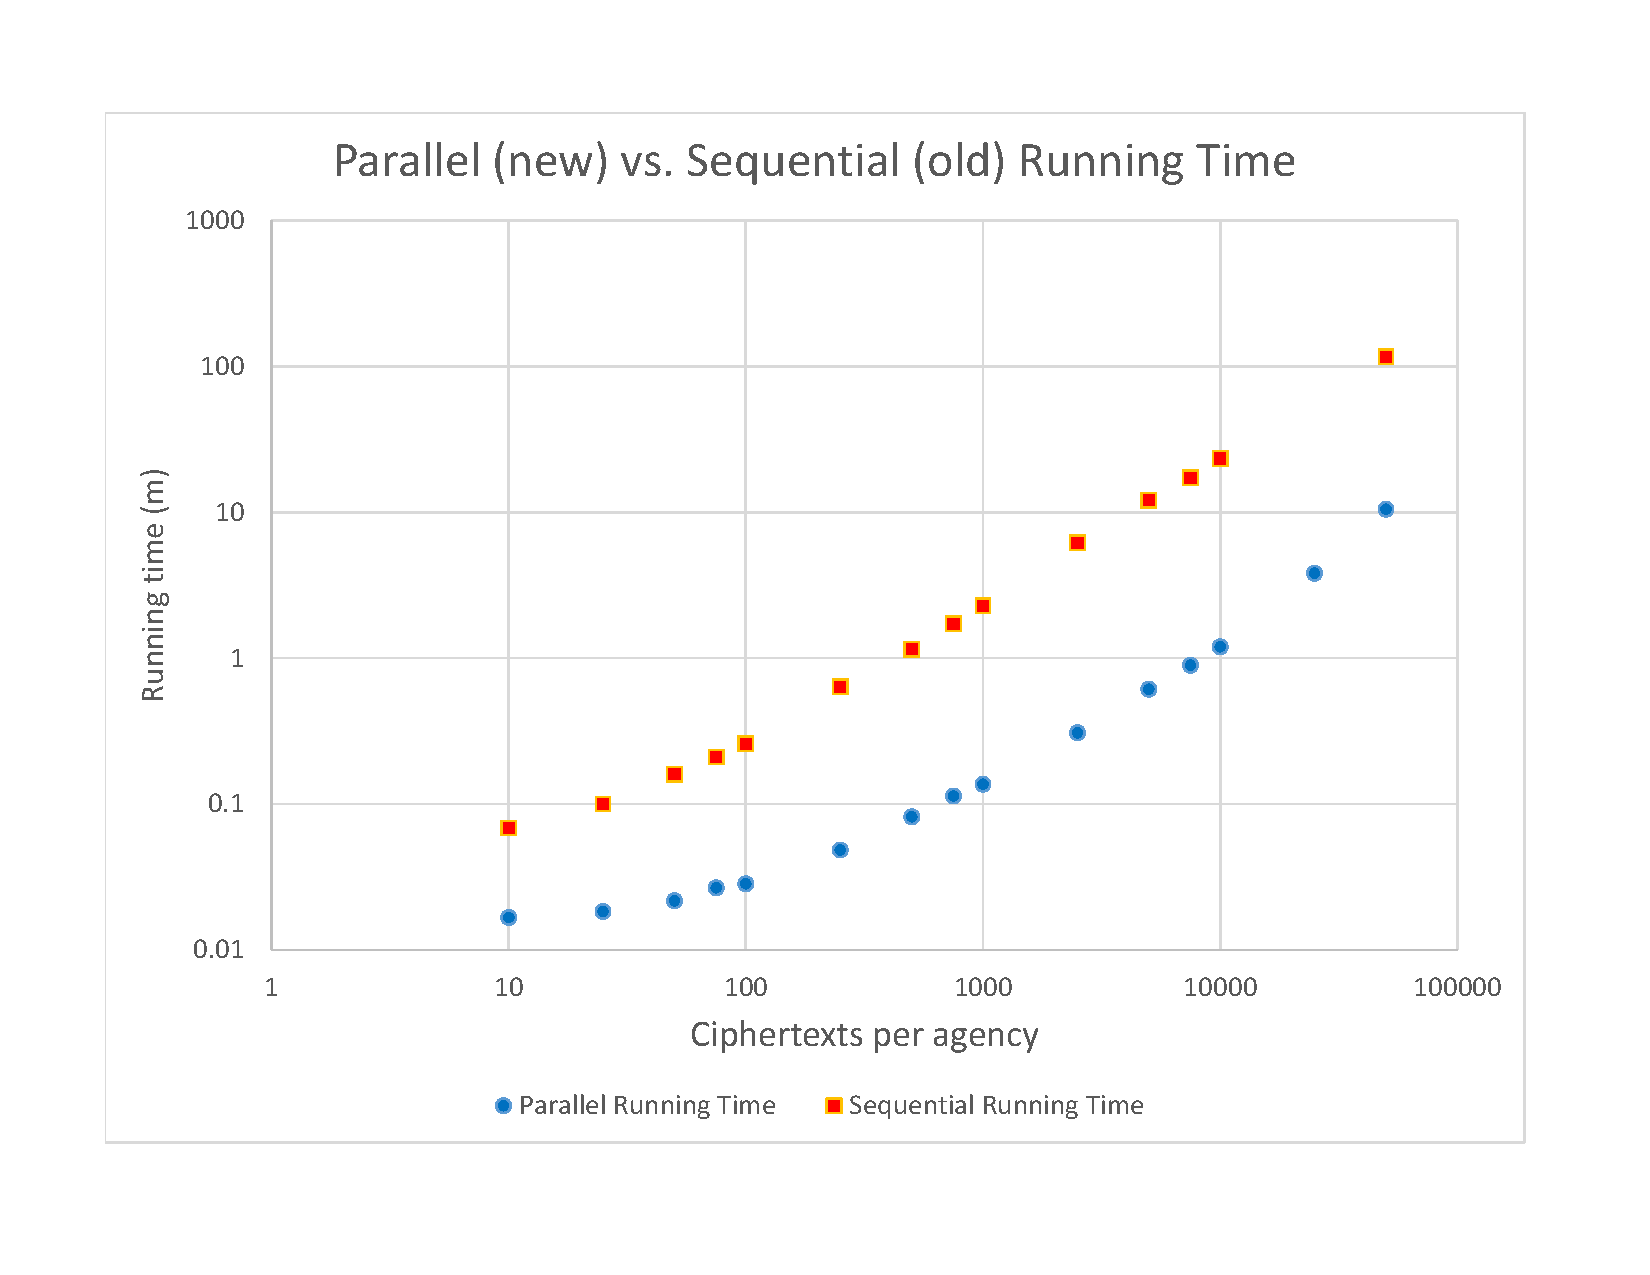
\includegraphics[width=0.99\columnwidth]{intersectionchart.pdf}
\caption{Comparison of Lawful Intersection Performance}
\label{fig:isectgraph}
\end{figure}

